\documentclass[conference]{IEEEtran}
\usepackage{amsmath,amssymb,booktabs,graphicx,multirow,tikz,balance,cite,url}
\usepackage{fontspec}
\setmainfont{Times New Roman}
\setsansfont{Arial}
\usepackage{caption}
\captionsetup{font=footnotesize,labelfont=normalfont,textfont=normalfont,labelsep=period}
\captionsetup[table]{position=bottom,skip=4pt,name=Table}
\renewcommand{\thetable}{\arabic{table}}
\usetikzlibrary{arrows.meta,positioning,fit}
\newcommand{\method}{LockPusher}
\title{LockPusher: State-Isolated World Models for Pushing under Joint Locks}
\author{Anonymous Authors}
\usepackage{placeins}

\setlength{\textfloatsep}{8pt plus 1pt minus 1pt}
\setlength{\dbltextfloatsep}{8pt plus 1pt minus 1pt}
\setlength{\dblfloatsep}{8pt plus 1pt minus 1pt}
\setlength{\floatsep}{8pt plus 1pt minus 1pt}
\setlength{\intextsep}{6pt plus 1pt minus 1pt}
\setcounter{topnumber}{3}
\setcounter{bottomnumber}{2}
\setcounter{totalnumber}{4}
\renewcommand{\topfraction}{.92}
\renewcommand{\bottomfraction}{.8}
\renewcommand{\textfraction}{.06}

\usepackage{balance,etoolbox}

\makeatletter
\providecommand{\bstctlcite}[1]{\@bsphack\immediate\write\@auxout{\string\citation{#1}}\@esphack}
\makeatother
\begin{document}
\bstctlcite{LPLayoutControl}
\twocolumn[{
\begin{@twocolumnfalse}
\maketitle
\begin{center}
\setlength{\abovecaptionskip}{3pt}
\setlength{\belowcaptionskip}{0pt}
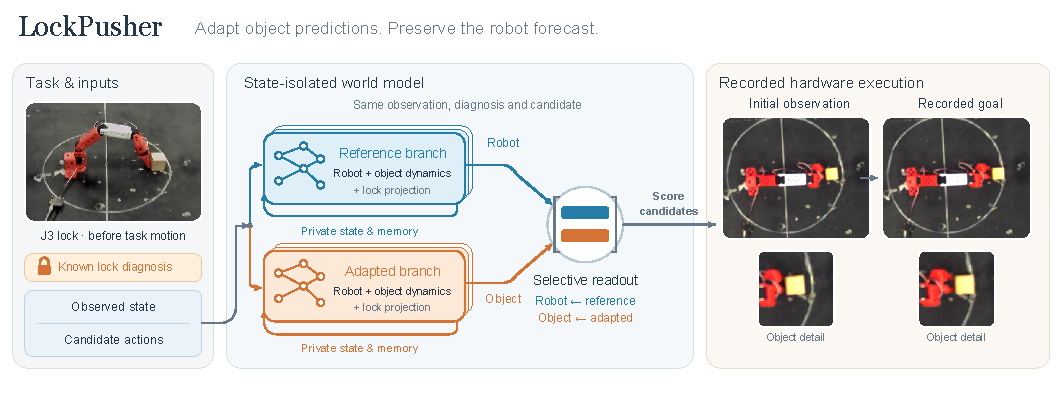
\includegraphics[width=\textwidth,trim=0 18pt 0 0,clip]{figures/teaser-arrow-20260915-194610/teaser.pdf}
\captionof{figure}{Overview of LockPusher's core idea and hardware execution. Given observed robot and object states, a diagnosed joint lock, and an object goal position, LockPusher selects contact actions to reposition the object without grasping. Left: task inputs and physical platform. Center: separate recurrent branches adapt object dynamics while preserving the reference robot forecast, combining both predictions to evaluate candidate pushes. Right: a J3-lock execution illustrates visual replanning toward the goal, with enlarged views showing object displacement.}\label{fig:overview}
\end{center}
\end{@twocolumnfalse}
}]
\begin{abstract}
Nonprehensile pushing enables robots to reposition objects that are difficult to grasp, but contact prediction becomes harder after a joint lock. Learned world models can adapt object dynamics from interaction data. In coupled recurrent models, however, an object correction may also change subsequent robot and pusher forecasts. We propose LockPusher, a state-isolated world model for diagnosed joint locks. An analytic projection imposes the lock constraint, while reference and intervention branches maintain separate states and memories and supply robot and object forecasts, respectively. For matched initial conditions and actions, robot and pusher forecasts remain equal to the projected reference at every deterministic rollout step. In a matched simulation benchmark, LockPusher achieves 1.58 mm object-position RMSE and 76.53\% task success, reducing prediction error by 46.98\% and improving success by 11.24 percentage points relative to the all-state residual baseline. Its advantage persists across the evaluated adaptation-data fractions. Historical paired ablations retain a 16.74\% mean reduction in composite object-state RMSE while preserving the reference forecast. On physical hardware, visual replanning completes all 18 trials across the intact arm and five single-joint locks, with a mean object endpoint error of approximately 1.64 pixels for a 40-pixel target displacement.
\end{abstract}
\begin{figure}[!tb]
\centering
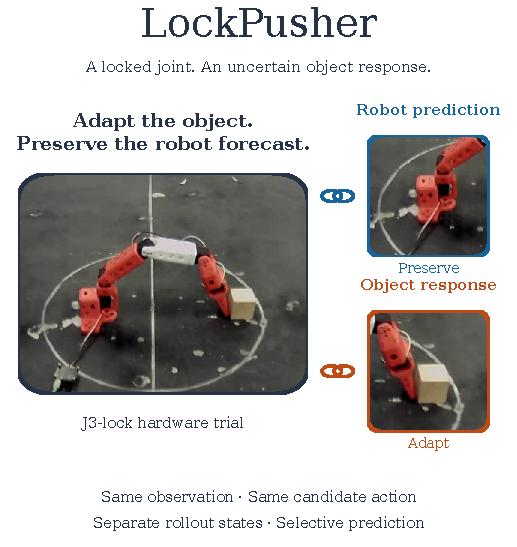
\includegraphics[width=.98\linewidth,trim=0 38 0 42,clip]{figures/lockpusher_teaser_dywa/lockpusher_poster.pdf}
\caption{Two key challenges addressed by LockPusher. During adaptation, the model must learn how a joint lock changes the object response to contact (object adaptation). During planning, it must retain the reference robot forecast while using the adapted object prediction to select candidate pushes (reference-preserving planning).}\label{fig:poster}
\end{figure}

\section{Introduction}
Nonprehensile manipulation extends a robot's ability beyond pick-and-place by moving objects that are difficult, undesirable, or impossible to grasp. Pushing is particularly useful in cluttered or constrained workspaces, but it is also contact rich: small errors in contact location, friction, or object response can accumulate over a rollout and change which candidate action appears most promising \cite{finn2017visual,bauza2018data}. Model-based planning addresses long-horizon decision making by predicting these outcomes before execution. Its usefulness therefore depends on a forward model that is accurate enough for action ranking and that respects the robot's available motion.

The overall task setting and the LockPusher execution interface are shown in Fig.~\ref{fig:overview}. This requirement becomes harder after a joint lock. A diagnosed lock supplies valuable information---the affected joint and its fixed angle---but it also changes the kinematic and dynamic context in which contact occurs. The robot must continue planning with fewer degrees of freedom, while the response of the pushed object remains uncertain. An analytic model can impose the known constraint, yet accurate contact prediction still depends on quantities such as friction and compliance that are difficult to specify. Learned world models reduce this burden by fitting interaction outcomes from data \cite{bauza2018data,kim2023se2}; damage-recovery methods instead adapt a policy or select compensatory behaviors \cite{cully2015robots,yang2021fault}. These two directions motivate a world model that can incorporate a diagnosed failure and adapt the uncertain object response used for planning.

The two design challenges addressed by LockPusher are summarized in Fig.~\ref{fig:poster}. Existing work improves different parts of this problem. Residual models correct approximate physics, and ActivePusher combines residual physics with uncertainty-guided data acquisition and planning \cite{zhong2026activepusher}. Dynamics-adaptive policies condition actions on interaction history to handle changing object and surface properties \cite{lyu2025dywa}. Fault-aware policies and behavior repertoires can recover task performance under disturbances or damage \cite{cully2015robots,yang2021fault}. Our concern is complementary: once an object correction is introduced into a recurrent world model, which predicted coordinates and internal memories are allowed to change?

This scope matters because robot and object predictions are coupled during rollout. The predicted robot state determines the pusher pose and may also be fed to a controller that generates the next candidate command. Consequently, an object correction fed back through a shared recurrence can change later robot states, pusher motion, and ultimately the action being scored. Restricting the immediate residual output to object coordinates does not remove this indirect path. Conversely, projecting the locked joint to its diagnosed angle guarantees the lock constraint but does not guarantee that the remaining robot forecast matches a chosen reference model. Our archived coupled-model evaluations expose this distinction: object-state error can decrease while free-state and pusher errors increase, even when diagnosed-lock violation is zero (Table~\ref{tab:historical-publication}).

We therefore formulate adaptation as an interface contract: update the object response while retaining a specified robot forecast for the same observation and candidate action. LockPusher combines analytic lock projection with state-isolated prediction. A reference branch, called the carrier, and an intervention branch receive the same projected inputs but maintain separate physical states and recurrent memories. The returned prediction takes robot coordinates from the carrier and object coordinates from the intervention branch, and this combined output is not fed back into either recurrence. For matched initial conditions and action sequences, the construction preserves the projected carrier robot and pusher trajectories at every deterministic rollout step while leaving the intervention branch free to model robot--object interaction and adapt the object forecast.

The adapted object predictions guide candidate selection: the planner ranks pushes by predicted terminal distance, executes part of the selected command, observes the scene again, and replans. We evaluate prediction and planning in a matched simulation benchmark, examine selective readout and recurrence in historical ablations, and test visual replanning on physical hardware. LockPusher achieves 76.53\% simulation success, exceeding Global by 11.24 percentage points, and completes all 18 hardware trials with a mean object endpoint error of approximately 1.64 pixels. The ablations separately test preservation of the reference forecast.

Our contributions are:
\begin{itemize}
\item A projected, state-isolated world model that permits object adaptation while preserving a specified robot forecast for matched inputs and action sequences.
\item Paired historical comparisons that separate object-prediction gains from collateral robot-prediction changes, together with a recurrence ablation of reference preservation.
\item A visual replanning system evaluated against two baselines in matched simulation and across 18 intact-arm and joint-lock hardware trials.
\end{itemize}

\section{Related Work}
\textbf{What changes during adaptation?} Prior work adapts different parts of the robot system: behaviour repertoires and robust policies compensate for damage or disturbances~\cite{cully2015robots,yang2021fault}; online factor estimation and control-oriented meta-learning support adaptation to changed dynamics~\cite{kumar2021rma,richards2021adaptive}; simulator tuning corrects physical parameters~\cite{allevato2020tunenet}. For pushing, recurrent and combined-prediction models update the object response from interaction history~\cite{cong2020self,gao2019online,li2018pushnet}. Building on these adaptation strategies, we impose an explicit output constraint: object corrections must retain a designated robot forecast for the same candidate action.

\textbf{How should contact dynamics be represented?} Pushing depends on friction, geometry, contact location, and speed~\cite{yu2016million}. Analytical sliding models~\cite{zhou2018convexpolynomial} and data-efficient learned predictors~\cite{bauza2018data,kim2023se2} offer complementary structure. Residual physics combines a nominal model with learned corrections in pushing and throwing~\cite{ajay2018augmenting,zeng2020tossingbot}; ActivePusher further links these corrections to active sampling and uncertainty-aware planning~\cite{zhong2026activepusher}. Relational models encode interacting entities~\cite{battaglia2016interaction,sanchezgonzalez2020learning}, with material adaptation in AdaptiGraph~\cite{zhang2024adaptigraph} and physical structure in PIN-WM~\cite{li2025pinwm}. LockPusher addresses a different design choice: which coordinates an object correction may change, and how that correction enters subsequent recurrence.

\textbf{How are predictions used for manipulation?} Visual foresight and neural dynamics support action evaluation and model-based learning~\cite{finn2017visual,nagabandi2018neural}. DyWA couples future-state and action prediction with history-based dynamics adaptation~\cite{lyu2025dywa}; structured world models learn affordance dynamics from human video~\cite{mendonca2023structured}. At execution time, hybrid MPC, online pushing models, and object-centric planning address contact modes and rearrangement~\cite{hogan2020reactive,wang2024unopush,ren2025objectcentric}, while HACMan learns contact locations and motions~\cite{zhou2023hacman}. Together with ActivePusher~\cite{zhong2026activepusher}, these works show how improved predictions guide manipulation. Our contribution concerns the prediction interface: reference robot and adapted object coordinates are combined for scoring, while each branch retains its own recurrent state. These methods establish the research context; our numerical comparison uses matched diagnosed-lock tasks and inputs.


\section{Problem Formulation}
\noindent\hspace*{1em}\textbf{Planning under a diagnosed lock.} Let $s=[r,o]\in\mathcal S$ denote the joint robot--object state, where $r=[q,\dot q]$ is the robot state and $o$ is the object state. The robot receives commands $a\in\mathcal A$. A diagnosis $d=(m,\bar q)$ specifies a binary joint-lock mask and the corresponding fixed angles. For a fixed diagnosis, we write the unknown discrete-time dynamics as
\begin{equation}
s_{t+1}=f_d^*(s_t,a_t).
\end{equation}
The diagnosis induces admissible states $\mathcal S_d$ and commands $\mathcal A_d$: locked joints remain at $\bar q$ with zero velocity and receive no command. Given an initial state $s_0$ and object goal region $\mathcal G$, the planning problem is to find a sequence $a_{0:H-1}\in\mathcal A_d^H$ whose trajectory remains admissible and reaches $o_H\in\mathcal G$. We study planar pushing with diagnosis available before planning. Contact dynamics are unknown, so candidate outcomes must be predicted from learned models~\cite{bauza2018data,cong2020self}.

\noindent\hspace*{1em}\textbf{Object-dynamics adaptation.} Let $\mathcal D$ collect observed interaction trajectories, each containing states $s_{0:H}$, actions $a_{0:H-1}$, and diagnosis $d$. A predictor uses these observations to approximate the outcomes of candidate actions. We distinguish the robot forecast from the object response because adaptation of a coupled recurrent model can change both, even when only the object prediction is intended to improve. Given a designated reference predictor $F_c$, our learning objective is to reduce object prediction error while preserving its robot forecast. For the same initial observation, diagnosis, and action sequence, the adapted predictor must satisfy
\begin{equation}
\hat r_t=\hat r_t^{\,c},\qquad t=1,\ldots,H,
\end{equation}
where $\hat r_t^{\,c}$ denotes the reference robot prediction after imposing the diagnosed constraint. This architecture-independent requirement covers both locked and free joints throughout the rollout.

\noindent\hspace*{1em}\textbf{Planning with a preserved robot forecast.} For each candidate $k$, the adapted model returns a trajectory $\hat s^{(k)}_{1:H}$ and terminal object position $\hat p_H^{(k)}$. Following predictive action evaluation~\cite{finn2017visual,hogan2020reactive}, our finite-candidate planner chooses
\begin{equation}
k^*=\arg\min_k\|\hat p_H^{(k)}-g\|_2,
\end{equation}
where $g$ is the target position. Thus, object adaptation may change the ranking of candidates while each retains its reference robot forecast. The preservation requirement specifies equality to $F_c$; prediction accuracy and task success are evaluated empirically. We therefore assess object prediction, preservation of the robot forecast, and the outcome of executed actions separately. The method below constructs a predictor that satisfies this requirement by design.

\section{Method}
LockPusher combines diagnosed constraints, object-dynamics adaptation, and candidate evaluation in a single prediction pipeline, as illustrated in Fig.~\ref{fig:isolation}. A reference branch and an adapted branch start from the same observation but maintain separate rollout states. The planner reads robot predictions from the reference and object predictions from the adaptation branch. We describe constraint projection, state isolation, the network implementation, training, and execution in turn.

\begin{figure*}[t]\centering
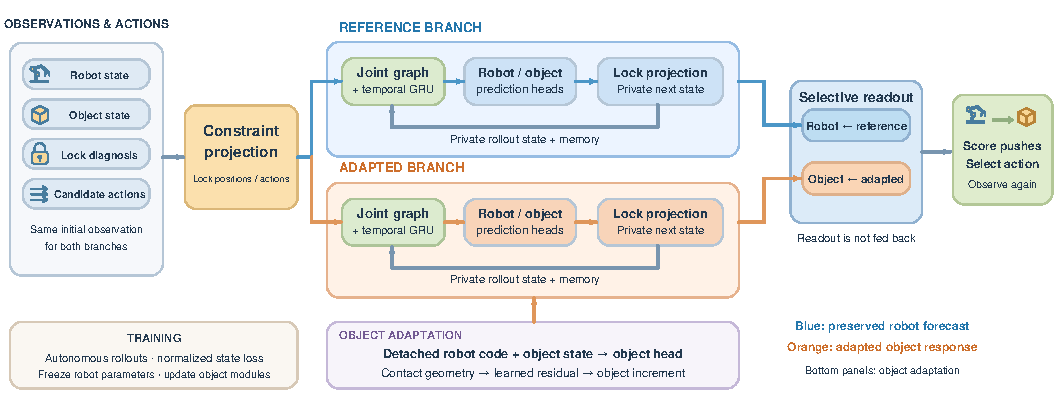
\includegraphics[width=.98\textwidth]{figures/lockpusher_revision/state_isolation.pdf}
\caption{LockPusher architecture. Constraint projection supplies both recurrent branches, which maintain private states and memories. Selective readout combines reference robot coordinates with adapted object coordinates for candidate scoring, without feedback into either branch. Detached robot features and contact geometry support object adaptation; the planner executes the selected action prefix and replans.}\label{fig:isolation}
\end{figure*}

\subsection{Incorporating the diagnosed lock}
LockPusher first incorporates the known constraint into prediction. For each joint $j$, define
\begin{align}
\Pi_d(q)_j&=(1-m_j)q_j+m_j\bar q_j,\\
\Pi_d(\dot q)_j&=(1-m_j)\dot q_j,\quad
\Pi_d(a)_j=(1-m_j)a_j.
\end{align}
Object coordinates are unchanged. Applying this projection to model inputs and predicted transitions keeps locked positions fixed and locked velocities zero throughout the rollout. Because $m_j$ is binary, applying the projection twice has the same effect as applying it once. Learned object adaptation therefore operates within an explicitly constrained robot prediction.


\subsection{Why rollout state must be isolated}
A one-step output mask does not, by itself, determine the behavior of a recurrent predictor. To see the distinction, consider a coupled transition with robot and object components $f_r,f_o$ and memory $h_t$. Suppose an adapted object value $\bar o_t$ is inserted into the next model input. Even when the current returned robot state is unchanged, the next prediction becomes
\begin{equation}
\bar r_{t+1}=f_r(r_t,\bar o_t,a_t,h_t).
\end{equation}
Relative to an unmodified object state $o_t$, the next robot difference is
\begin{equation}
\Delta r_{t+1}=f_r(r_t,\bar o_t,a_t,h_t)
-f_r(r_t,o_t,a_t,h_t).
\end{equation}
Object changes can propagate through both the state and recurrent memory, affecting future robot outputs. The magnitude and effect of this feedback depend on the coupled model.

LockPusher removes this feedback path at the rollout interface. Each branch advances its own state and memory. The combined state supplies candidate evaluation, while recurrence uses the private branch states. Both branches may still contain robot--object interactions internally. Isolation controls state exchange between predictors while retaining robot--object interactions within each branch.

The deployed block-structured model is a special case: its robot transition does not consume object state. In that configuration, object-only updates can already preserve robot predictions when robot parameters and inputs remain fixed. State isolation supplies the explicit interface contract and also applies to historical coupled predictors. Distinguishing these configurations is necessary when interpreting the recurrence comparisons: a preservation test on a coupled model and an object-adaptation test on the deployed architecture answer different questions.

\subsection{Object adaptation with separate rollout states}
The carrier $F_c$ supplies the reference prediction. An intervention model $F_i$ supplies the adapted object response. Each branch maintains its own physical state $s^b_t$ and recurrent state $h^b_t$, where $b\in\{c,i\}$. Starting from the same projected observation, both branches receive the same projected candidate action:
\begin{align}
(s^b_{t+1},h^b_{t+1})&=F_b(s^b_t,\Pi_d(a_t),d,h^b_t),\\
s^b_{t+1}&\leftarrow\Pi_d(s^b_{t+1}),\\
\hat s_{t+1}&=[r^c_{t+1},o^i_{t+1}].\label{eq:publish}
\end{align}
The returned state combines the two predictions for scoring. Private recurrence preserves the reference rollout while allowing the intervention to propagate its learned object dynamics.

\textbf{Reference-trajectory preservation.} For deterministic branches with matched initial states, carrier parameters, diagnoses, and candidate actions, the returned robot trajectory equals the standalone projected carrier trajectory at every step. The initial carrier states agree. If they agree at step $t$, the same transition, hidden state, action, and projection produce the same next state. Equation~\eqref{eq:publish} returns that carrier state, establishing the result by induction. The pusher trajectory is also preserved because it is computed from joint positions by the same forward kinematics. For fixed candidates, deterministic evaluation terms computed solely from robot coordinates are also preserved. This property is relative to the chosen carrier; prediction accuracy and joint dynamical consistency are separate properties.

\subsection{Contact-conditioned object adaptation}
A joint lock changes the relation between robot motion and object response. We therefore condition object corrections on explicit contact geometry, complementing the learned robot representation~\cite{ajay2018augmenting,zhong2026activepusher}. Let $z_t$ denote robot features and $\phi_t$ describe pusher motion, relative object geometry, object velocity, and contact proximity. The adapted transition is
\begin{equation}
o_{t+1}=o_t+G_\theta([\operatorname{sg}(z_t),o_t])+R_\psi(\operatorname{sg}(\phi_t)).
\end{equation}
The object head $G_\theta$ captures the nominal response; $R_\psi$ learns geometry-dependent corrections. Stop-gradient retains the predictive value of robot features while directing adaptation to the object modules. Contact proximity is encoded as $\gamma_{\ell,t}=\sigma((\tau-c_{\ell,t})/\epsilon)$, where $c_{\ell,t}$ is the clearance at rollout stage $\ell$, $\tau$ is a distance offset, and $\epsilon>0$ controls smoothness. These features allow the residual to respond to changes in contact configuration. Independent recurrence then propagates the adapted object dynamics while maintaining the reference robot trajectory.



\subsection{Matched adaptation}
For the large-scale adaptation study, all variants start from the same pretrained carrier. We freeze its robot parameters and update the object head. LockPusher additionally updates its geometric object residual. The no-residual variant excludes this correction, while the global variant learns corrections to all state coordinates. All variants use the same data and optimization budget.

The underlying adaptation model is trained directly. Its predictions $\tilde s_t$ minimize normalized squared state errors over an autonomous prediction window; state isolation is applied when returning candidate predictions:
\begin{equation}
\mathcal L=\frac{1}{d_s H}\sum_{t=1}^{H}\|D^{-1}(\tilde s_t-s_t)\|_2^2.
\end{equation}
The diagonal matrix $D$ normalizes state coordinates. Robot parameters are fixed during object adaptation; the global baseline also adapts robot coordinates.


The scales in $D$ are fixed across variants. The validation-selected model is frozen for closed-loop evaluation.

\par\smallskip\noindent
\begin{minipage}{\linewidth}
\hrule height 0.4pt\smallskip
\textbf{Algorithm 1: Object-dynamics adaptation}\label{alg:adaptation}\\
\textbf{Input:} Pretrained model $F_0$, training/validation data, scale $D$, epochs $E$, horizons $H_e,H_v$.\\
\textbf{Output:} Validation-selected adapted model $F_i$.
\smallskip\hrule height 0.4pt\smallskip
\begin{tabular}{@{}r@{\quad}p{.87\linewidth}@{}}
1 & Initialize $F_i\leftarrow F_0$; freeze robot parameters.\\
2 & Retain the initial model as a validation candidate.\\
3 & \textbf{for} epoch $e=1,\ldots,E$ \textbf{do}\\
4 & \quad Set rollout horizon $H\leftarrow H_e$.\\
5 & \quad Sample one contiguous window per training trajectory.\\
6 & \quad Roll out $F_i$ autonomously from each initial state.\\
7 & \quad Update object head and residual using $\mathcal L$.\\
8 & \quad Evaluate horizon-$H_v$ object-position MSE.\\
9 & \textbf{return} checkpoint with lowest validation MSE.
\end{tabular}
\smallskip\hrule
\end{minipage}\par\smallskip

\subsection{Candidate selection and execution}
A new observation reinitializes both branches after execution. Simulation executes action commands; hardware moves toward selected joint references. The experiment section reports the candidate counts and execution settings.


For $K$ candidates and horizon $H$, each branch requires $KH$ transitions. Candidates can be batched independently; each maintains its own temporal recurrence. The two-branch construction adds a reference rollout to the intervention rollout. Preservation applies to each matched candidate. Adaptation can change the selected action through its effect on predicted object outcomes.


\par\smallskip\noindent
\begin{minipage}{\linewidth}
\hrule height 0.4pt\smallskip
\textbf{Algorithm 2: State-isolated candidate evaluation}\label{alg:rollout}\\
\textbf{Input:} Observation $s_0$, diagnosis $d$, goal $g$, candidates $\mathcal U$, branches $F_c,F_i$.\\
\textbf{Output:} Selected sequence $a^{(k^*)}_{0:H-1}$.
\smallskip\hrule height 0.4pt\smallskip
\begin{tabular}{@{}r@{\quad}p{.87\linewidth}@{}}
1 & \textbf{for each} candidate $a^{(k)}\in\mathcal U$ \textbf{do}\\
2 & \quad Initialize both branches at $\Pi_d(s_0)$ with their own initial memories.\\
3 & \quad \textbf{for} $t=0,\ldots,H-1$ \textbf{do}\\
4 & \qquad $u_t\leftarrow\Pi_d(a_t^{(k)})$\\
5 & \qquad Update $(s^b,h^b)$ independently, $b\in\{c,i\}$.\\
6 & \qquad Project each state: $s^b\leftarrow\Pi_d(s^b)$.\\
7 & \qquad Return $[r^c,o^i]$ without branch feedback.\\
8 & \quad $\hat c_k\leftarrow\|\hat p_H^{(k)}-g\|_2$\\
9 & \textbf{return} sequence indexed by $\arg\min_k\hat c_k$.
\end{tabular}
\smallskip\hrule
\end{minipage}
\par\smallskip

\section{Experiments}
\label{sec:experiments}
We evaluate three questions: whether restricted adaptation improves object prediction and closed-loop planning across adaptation-data budgets under diagnosed joint locks; whether selective readout and independent recurrence retain object corrections while preserving the reference robot forecast; and whether the controller completes pushes under physical joint locks.




\subsection{Simulation benchmark and quantitative comparison}
\noindent\hspace*{1em}\textbf{Task setup.} We evaluate planar box pushing under five single-joint locks in MuJoCo~\cite{todorov2012mujoco}. The object has a fixed orientation. Dynamics settings comprise nominal conditions, doubled damping, 70\% actuator gain, and the combination of the latter two. Each trajectory starts from an independent reset with checks on support geometry and joint limits. Training, validation, and test sets contain 50,000, 2,000, and 6,000 trajectories, respectively.

\noindent\hspace*{1em}\textbf{Implementation and training.} The robot encoder uses a five-node chain graph~\cite{battaglia2016interaction,sanchezgonzalez2020learning}, hidden width 136, two message-passing rounds and 136-unit GRUs~\cite{cho2014gru}. SiLU~\cite{elfwing2018silu} networks have widths $6\to136\to136$ (encoder), $272\to136\to136$ (messages), $136\to136\to2$ (joint head), and $140\to136\to4$ (object head). The residual uses a 12-dimensional descriptor and a 16-unit Tanh hidden layer. Its inputs are previous/next pusher positions, their difference, next-pusher-to-object displacement, object velocity, and pre/post-transition contact gates. Capsule radii are 12 and 8 mm; the object box is 40 mm; $\tau=-0.005$ m and $\epsilon=0.002$ m. The state dimension is $d_s=14$. Normalization scales are 0.1 rad, 1 rad/s, 0.03 m, and 0.1 m/s for joint position/velocity and object position/velocity. Training uses $E=10$ epochs, with $H_e=10$ for the first five and $H_e=25$ thereafter; each trajectory supplies one random contiguous window per epoch. Validation uses $H_v=25$, including the initial checkpoint.

\noindent\hspace*{1em}\textbf{Baselines.} We compare three adaptation variants of the same pretrained model to evaluate the effect of adaptation scope. Carrier adapts the object head with robot parameters fixed; LockPusher adds a geometric object residual while retaining the reference robot forecast; Global permits residual corrections to all state coordinates. The methods share pretrained weights, data, optimization budgets, and adaptation seeds 7, 17, and 27. Checkpoints are selected by 25-step validation object-position error. This comparison tests the contribution of the object residual and the effect of also adapting robot coordinates.

\noindent\hspace*{1em}\textbf{Evaluation protocol.} All methods solve the same 1,200 initial-state--goal problems, with a mean initial goal distance of 65 mm. Each planning cycle selects among 128 candidates, executes ten steps, and obtains a new observation. Five cycles give 0.25 s of execution. We report per-coordinate object-position RMSE at step 50, mean final goal distance, and the fraction of trials with a final goal distance of less than 1 mm. The matched full-data comparison is summarized in Table~\ref{tab:core-results}.

\begin{table}[!tbp]\centering\small

\setlength{\tabcolsep}{4pt}
\begin{tabular}{lrrr}\toprule
Method & \shortstack{Object RMSE\\(mm)} & \shortstack{Goal distance\\(mm)} & \shortstack{Success\\(\%)}\\\midrule
Carrier &5.07&3.32&47.84\\
Global &2.98&2.06&65.29\\
LockPusher &\textbf{1.58}&\textbf{1.43}&\textbf{76.53}\\\bottomrule
\end{tabular}\caption{Full-data simulation results averaged over three training seeds. LockPusher achieves lower prediction and goal errors and higher task success than both baselines. RMSE denotes root mean squared error.}
\label{tab:core-results}
\end{table}
\noindent\hspace*{1em}\textbf{Results.} LockPusher achieves 1.58 mm object-position RMSE, 1.43 mm final goal distance, and 76.53\% success. Relative to Global, prediction error decreases by 46.98\% and success increases by 11.24 percentage points. Thus, restricting robot-side adaptation can accompany improved object prediction and closed-loop task performance in this benchmark.



\noindent\hspace*{1em}\textbf{Effect of adaptation-data budget.} We evaluate ten adaptation-data fractions from 10\% to 100\% and retain the same evaluation tasks at each fraction. Figure~\ref{fig:adaptation-data}(a,c,e) reports the mean and one standard deviation over three training seeds. LockPusher achieves lower mean object-position RMSE and final goal distance, together with higher mean task success, at every evaluated fraction. Its simulation advantage therefore extends across the tested adaptation budgets.

\begin{figure}[!tb]
\centering
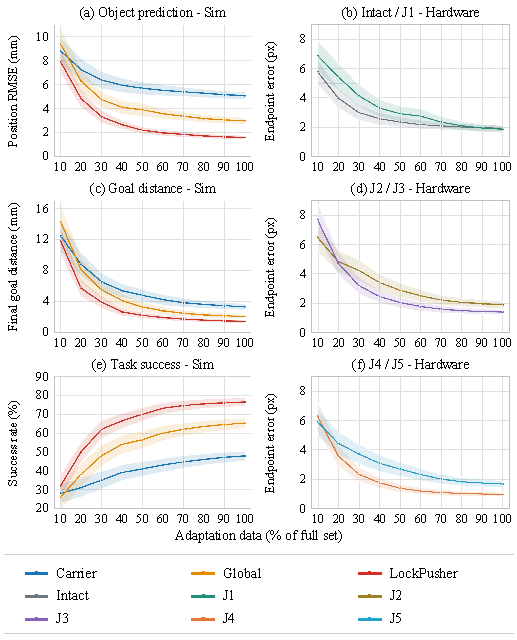
\includegraphics[width=\columnwidth]{figures/submission-layout-20260915-191848/adaptation_data_single_column.pdf}
\caption{LockPusher improves simulation prediction and task performance across the tested data budgets (left); hardware endpoint error decreases as adaptation data increase (right). Shading shows mean $\pm1$ SD over three training seeds. Hardware 100\% denotes 100 adaptation trajectories per condition.}
\label{fig:adaptation-data}
\end{figure}

\begin{figure*}[!t]
\centering
\includegraphics[width=\textwidth]{figures/lockpusher_revision/all18_oblique.pdf}
\caption{LockPusher performs nonprehensile pushing with the intact arm and under five single-joint locks. Three recorded executions per condition illustrate its ability to continue object manipulation with different joints immobilized.}
\label{fig:hardware-oblique}
\end{figure*}

\subsection{Module analysis and ablations}
\noindent\hspace*{1em}\textbf{Object adaptation and reference preservation.} We test whether selective readout and independent recurrence retain object corrections while controlling their effect on robot predictions. With fixed checkpoints and paired inputs, the two experiments change the returned coordinates and the rollout feedback, respectively.

\noindent\hspace*{1em}\textbf{Effect of selective readout.} Using the same historical checkpoints, we compare full-state intervention and selective readout. Both readouts use the same object prediction, so both retain the 16.74\% mean reduction in composite object-state RMSE; they differ in the robot coordinates returned to the planner. Full-state intervention reduces free-state error in 24 combinations and increases it in three, by up to 6.20\%. Selective readout retains Carrier's free-state and pusher errors in all 27 combinations (Table~\ref{tab:historical-publication}).

\begin{table}[!tbp]\centering\small

\setlength{\tabcolsep}{3pt}
\begin{tabular}{lrrrr}\toprule
& \shortstack{Object RMSE\\reduction (\%)} & \shortstack{Free\\worse} & \shortstack{Max. free\\increase (\%)} & \shortstack{Free/FK\\match}\\\midrule
Carrier & 0.00 & 0/27 & 0.00 & 27/27\\
Full-state & 16.74 & 3/27 & 6.20 & 0/27\\
Selective & 16.74 & 0/27 & 0.00 & 27/27\\
\bottomrule\end{tabular}\caption{Historical selective-readout ablation across 27 combinations. Both readouts retain the same object-error reduction, while selective readout preserves the reference robot prediction in every combination. Free worse counts increased free-state errors; Free/FK match counts unchanged free-state and forward-kinematics pusher errors. Changes are relative to Carrier.}
\label{tab:historical-publication}
\end{table}
\noindent\hspace*{1em}\textbf{Effect of independent recurrence.} We fix weights and inputs and compare shared-state feedback with independent recurrence on 12 trajectories in each of seven conditions, totaling 84 trajectories. Three checkpoints, seven conditions, and horizons of 10, 25, and 50 steps give 63 evaluation combinations. Independent recurrence preserves the reference robot prediction in all 63 combinations, whereas shared feedback changes it in all 63; object-position and velocity RMSE are identical. Robot error decreases in 60 combinations and increases in three. The historical reset protocol awaits independent physical-validity checks.




\subsection{Real-world experiments}
\noindent\hspace*{1em}\textbf{Hardware setup.} The hardware platform and recorded intact-arm and joint-lock executions are shown in Figs.~\ref{fig:real-scene} and~\ref{fig:hardware-oblique}; for the deployed controller, we execute three pushes on the intact arm and under each of the J1--J5 locks, for 18 trials. Each target displacement is 40 image pixels, approximately 51.2 mm under the calibration used for this batch. The controller uses the seed-27 deployment weights and evaluates at least 10,000 joint-reference sequences over 50 steps. It executes the selected reference with a 5-degree/s speed limit and replans from a new observation. Repetitions within each condition reuse a preparation candidate set.
\begin{figure}[!t]\centering
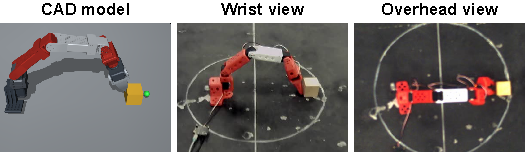
\includegraphics[width=\columnwidth]{figures/hardware-aligned-20260915-200334/environment_plate.pdf}
\caption{We impose joint locks on the same physical arm and record nonprehensile pushing with wrist and overhead cameras.}\label{fig:real-scene}
\end{figure}


\noindent\hspace*{1em}\textbf{Evaluation.} Figure~\ref{fig:hardware-sequence} illustrates the image-space criterion. A trial succeeds when target error is at most two pixels on each image axis in three distinct, consecutive reliable frames. Object endpoint error is computed separately as the norm of the coordinate-wise median XY error over the final ten frames. Table~\ref{tab:hardware-scores} reports both object endpoint error and task outcomes.
\begin{figure}[!t]\centering
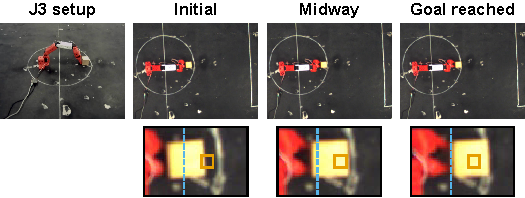
\includegraphics[width=\columnwidth]{figures/hardware-aligned-20260915-200334/hardware_sequence.pdf}
\caption{Under a J3 joint lock, our controller uses visual replanning to push the object toward its goal and confirms arrival through the center-point error in three consecutive frames.}\label{fig:hardware-sequence}
\end{figure}


\begin{table}[!tbp]\centering\small

\begin{tabular}{lrr}\toprule
Condition & \shortstack{Object endpoint error\\mean (px)} & Successes/trials\\\midrule
Intact &1.94&3/3\\
J1 &1.88&3/3\\
J2 &1.92&3/3\\
J3 &1.43&3/3\\
J4 &0.97&3/3\\
J5 &1.68&3/3\\
\midrule All &1.64&18/18\\\bottomrule
\end{tabular}\caption{Real-world results for 40-pixel target displacements. Each success entry gives successful trials out of three attempts. LockPusher completes all tested pushes across the intact arm and five joint-lock conditions; endpoint errors are condition means in pixels.}
\label{tab:hardware-scores}
\end{table}


\noindent\hspace*{1em}\textbf{Pushing under joint locks.} The intact arm and all five single-joint-lock conditions complete three pushes each, giving 18 successful trials. Mean object endpoint error is approximately 1.64 pixels, with condition means from 0.97 to 1.94 pixels. 

The same data-budget study continues on hardware: we collect 100 complete adaptation trajectories for each of the intact-arm and five joint-lock conditions, totaling 600 trajectories. Each fraction uses 10--100 trajectories from its own condition and is evaluated on the same test tasks. Figure~\ref{fig:adaptation-data}(b,d,f) reports means and one standard deviation over three training seeds. Mean object endpoint error decreases as adaptation data increase in all six conditions, extending the simulation trend to physical execution. 





\section{Conclusion and future work}
We presented LockPusher, a world-model framework for nonprehensile pushing under diagnosed joint locks. By separating the reference robot forecast from adapted object dynamics, LockPusher learns contact-response changes while preserving the robot forecast for each candidate action, and uses the adapted object prediction to guide pushing. Simulation shows lower prediction error and higher task success across the evaluated adaptation budgets. Hardware experiments demonstrate pushing with the intact arm and under five single-joint locks. This combination provides an explicit interface for contact planning with motion-restricted robots.

The formulation assumes a known lock diagnosis and a fixed-orientation planar object, making admissible motion and contact geometry explicit. Its central principle defines the scope of adaptation: object response is updated while a designated robot forecast is preserved throughout recurrence. Future work will address object rotation, diverse contact geometries, changing robot dynamics, and constraints that balance robot-prediction updates with planning consistency.

\bibliographystyle{IEEEtran}
\bibliography{references-complete-20260915-194900}
\end{document}




